\section{归一化拉普拉斯}
\label{sec:graph-normalized-laplacian}

前面几节讨论的组合拉普拉斯矩阵$\bm L=\bm D-\bm W$在标准欧氏内积下给每个顶点相同的单位权重$1$。它可描述以边权为跳转速率的连续时间扩散；若采用每步跳转一次、按边权比例选择邻居的离散随机游走，则应使用按度归一化的算子。两种模型的时间尺度不同。下面通过两个例子说明归一化的作用（图~\ref{fig:laplacian-diffusion-bottleneck}）。

第一个例子是图~\ref{fig:laplacian-diffusion-bottleneck}(a)所示的“双团哑铃图”：两个各含$m$个顶点的稠密完全图团$K_m$之间仅通过一条单位权桥边$u\!-\!v$相连。在桥端点$u$处，共有$m-1$条边连向同侧团内部，只有$1$条桥边连向对侧团（度数为$d_u=m$）。当一个随机游走粒子到达$u$时，它在下一步等概率地从$m$条关联边中任选一条迈出，因此只有$\frac{1}{m}$的概率跨过桥边进入右侧团，而有$\frac{m-1}{m}$的概率退回左侧团内部。当团规模$m$很大时，尽管桥边的绝对权重仍为$1$，粒子在桥端点跨团转移的概率却因团内邻接边增多而降为$\frac{1}{m}$，全图的跨团混合速度随团规模增大而变慢。

第二个例子是图~\ref{fig:laplacian-diffusion-bottleneck}(b)所示的含高连接度枢纽的网络：中心枢纽顶点$h$连接了$D\gg 1$条边，而右侧普通顶点$i$只连接$2$条边。粒子从普通顶点$i$出发时，每条关联边分到$\frac{1}{2}$的转移概率；而从枢纽顶点$h$出发时，每条边分到的转移概率$w_{h,j}/d_h$为$\frac{1}{D}$。

若把全图所有边权同时乘以$10$，每个正度顶点按权重比例选择邻居的转移概率$w_{i,j}/d_i$保持不变，离散随机游走也保持不变；组合拉普拉斯及其特征值则乘以$10$，对应连续时间扩散加速$10$倍。若只缩放局部边权，边界顶点的转移概率一般会改变，不能作相同推断。

\begin{BookInlineFigure}
  \centering
  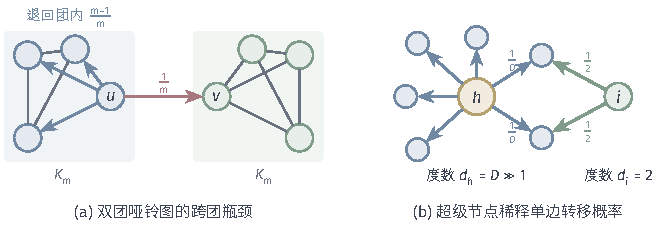
\includegraphics[width=111.633mm]{figures/03-graphs/05-matrices-and-spectra/tikz/laplacian-diffusion-bottleneck/figure.pdf}
  \caption{度数分布对一步随机游走转移概率的稀释效应。（a）双团哑铃图中，桥端点$u$有$m-1$条团内边和$1$条跨团桥边，粒子跨过桥边的概率仅为$1/m$，以$(m-1)/m$的概率退回原团。（b）度数为$D\gg 1$的枢纽顶点$h$将每条关联边上的转移概率稀释为$1/D$，而度数为$2$的普通节点$i$在每条边上分配$1/2$的转移概率。}
  \label{fig:laplacian-diffusion-bottleneck}
\end{BookInlineFigure}

在每步跳转一次的离散随机游走模型中，转移概率取决于边权占顶点加权度的比例，跨区瓶颈则与割权占集合体积$\operatorname{vol}(S)=\sum_{i\in S}d_i$的比例有关。归一化谱与这一时间尺度相适应。

为研究上述离散随机游走，使用度矩阵$\bm D$对拉普拉斯矩阵作归一化。本节先引入以度数计权的度加权内积与集合体积，再分别构造对称归一化拉普拉斯$\mathcal L=\bm D^{-1/2}\bm L\bm D^{-1/2}$和随机游走拉普拉斯$\bm L_{\mathrm{rw}}=\bm D^{-1}\bm L$，对比两种归一化算子的联系与分工，最后证明归一化拉普拉斯谱的性质。

\subsection{度加权内积}
\label{sec:graph-degree-weighted-inner-product}

标准欧氏长度平方$\sum_i x_i^2$给每个顶点相同的权重$1$。为了按每个顶点的连接量计权，将第$i$个坐标的权重替换为该顶点的加权度$d_i$，在正度顶点集$V_+=\{i\in V:d_i>0\}$上定义\term{度加权内积}（degree-weighted inner product）及其诱导范数：
\begin{equation}
  \langle \bm x,\bm y\rangle_{\bm D}
  =\bm x^\top\bm D\bm y
  =\sum_{i\in V_+}d_i\,x_iy_i,
  \qquad
  \lVert\bm x\rVert_{\bm D}^2=\bm x^\top\bm D\bm x.
  \label{eq:graph-degree-weighted-inner-product}
\end{equation}
在$V_+$上所有$d_i>0$，故任意非零向量的度加权长度平方$\lVert\bm x\rVert_{\bm D}^2>0$，式~\eqref{eq:graph-degree-weighted-inner-product}确实构成$V_+$上的内积。

用度加权范数衡量单点脉冲$\bm e_i$（$i\in V_+$）时，其沿边变化能量为$\bm e_i^\top\bm L\bm e_i=d_i$，度加权长度平方同样为$\lVert\bm e_i\rVert_{\bm D}^2=d_i$，两者之比对任意正度顶点都恒等于
\[
  \frac{\bm e_i^\top\bm L\bm e_i}{\lVert\bm e_i\rVert_{\bm D}^2}=\frac{d_i}{d_i}=1.
\]
例如在四点五边单位权图上，度为$3$的顶点$1$与度为$2$的顶点$2$在标准欧氏范数下的单位脉冲能量分别为$3$和$2$，而在度加权范数下，每单位连接量所承担的变化比值完全一致，均为$1$。

将任意顶点子集$S\subseteq V$的指示向量$\bm 1_S$代入度加权长度平方，立得子集内各顶点的加权度总和：
\begin{equation}
  \operatorname{vol}(S)=\sum_{i\in S}d_i
  =\lVert\bm1_S\rVert_{\bm D}^2.
  \label{eq:graph-laplacian-vertex-volume}
\end{equation}
这个和称为顶点子集$S$的\emph{体积}（volume），它精确计量了$S$所关联的边权容量：两端都在$S$内部的边在两个端点各计一次共两倍权重，跨出$S$的边计一倍权重。例如四点五边图中$S=\{1,2\}$的体积为$d_1+d_2=3+2=5$。

结合第~\ref{sec:graph-laplacian-energy}节的割权公式$\bm 1_S^\top\bm L\bm 1_S=c(S,V\setminus S)$，指示向量$\bm 1_S$的度加权Rayleigh商为
\[
  \frac{\bm 1_S^\top\bm L\bm 1_S}{\bm 1_S^\top\bm D\bm 1_S}
  =\frac{c(S,V\setminus S)}{\operatorname{vol}(S)}.
\]
这一比值直接给出了切开$S$的跨割边权重占$S$总连接体积的比例——这正是第~\ref{chap:spectral-partition}章导通率与归一化割（NCut）的核心度量。

需要注意，孤立顶点的加权度$d_i=0$，一个只在孤点上取$1$的非零向量在$\bm x^\top\bm D\bm x$下得零值，因此在包含孤点的全空间上$\sqrt{\bm x^\top\bm D\bm x}$只是半范数，相应双线性型不构成正定内积。下面的推导先在正度顶点集$V_+$上进行，再约定孤点在全空间矩阵中的零扩展。

\subsection{对称归一化拉普拉斯}
\label{sec:graph-symmetric-normalized-laplacian}

在$V_+$上，一组读数的能量与度加权长度平方之比为
\[
  \frac{\bm x^\top\bm L\bm x}{\bm x^\top\bm D\bm x},
  \qquad \bm x\ne\bm0.
\]
这是一个广义 Rayleigh 商。如果能把分母变成普通欧氏长度平方，就可以直接使用对称矩阵的谱分析工具。

观察分母中的每一项$d_ix_i^2$。它可以写成$(\sqrt{d_i}\,x_i)^2$。这就提示我们引入新坐标$y_i=\sqrt{d_i}\,x_i$。在正度顶点上，这个变换是可逆的：$x_i=y_i/\sqrt{d_i}$。新坐标描述的仍然是同一组读数，只是数值按度的平方根缩放了。

以四点图上的常值读数$x_i=1$为例。顶点$1$和$3$的度为$3$，对应新坐标为$\sqrt3$。顶点$2$和$4$的度为$2$，对应新坐标为$\sqrt2$。尽管四个新坐标的数值不同，还原后的实际读数仍然处处相等。

将$\bm x=\bm D^{-1/2}\bm y$代入分子，左右各出现一个$\bm D^{-1/2}$：
\[
  \bm x^\top\bm L\bm x
  =\bm y^\top(\bm D^{-1/2}\bm L\bm D^{-1/2})\bm y.
\]
分母已经变成$\bm y^\top\bm y$。整个比值成为新坐标上一个对称矩阵的普通 Rayleigh 商。矩阵极值性质可参考\BookChapterRef{chap:matrix-approximation}{卷二"矩阵逼近"章}。

\begin{definition}[对称归一化拉普拉斯]
\label{def:graph-symmetric-normalized-laplacian}
在正度顶点上，\term{对称归一化拉普拉斯}（symmetric normalized Laplacian）定义为
\begin{equation}
  \begin{aligned}
  \mathcal L&=\bm D^{-1/2}\bm L\bm D^{-1/2}\\
            &=\bm I-\bm D^{-1/2}\bm W\bm D^{-1/2}.
  \end{aligned}
  \label{eq:graph-symmetric-normalized-laplacian}
\end{equation}
含孤点时，在$\bm D^{-1/2}$中将孤点位置取零，用第一式定义全空间上的矩阵。
\end{definition}

在新坐标中，一条边比较的是$y_i/\sqrt{d_i}$和$y_j/\sqrt{d_j}$，即还原后的实际读数。因此，原读数在某个连通分量上取常值$1$、分量外取$0$时，新坐标中的零方向变为$\bm D^{1/2}\bm1_{V_a}$，即各点取$\sqrt{d_i}$。图~\ref{fig:laplacian-degree-coordinates}展示了四点图上常值读数的两种坐标。右图中四个坐标因度而异，但还原为实际读数后各边差值仍为零。

\begin{BookInlineFigure}
  \centering
  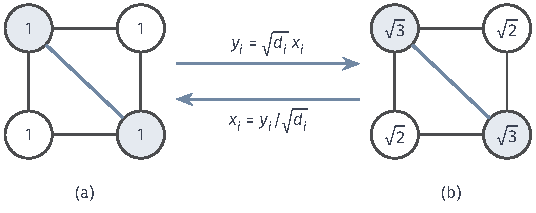
\includegraphics{figures/03-graphs/05-matrices-and-spectra/tikz/laplacian-degree-coordinates.pdf}
  \caption{同一组常值读数的两种坐标。浅蓝顶点度为三，白色顶点度为二。（a）原读数都为一。（b）按度的平方根缩放后，坐标因度而异。计算边差时，先按下方箭头把每个坐标还原。}
  \label{fig:laplacian-degree-coordinates}
\end{BookInlineFigure}

现在把孤点放回全空间。规定孤点在矩阵中有一行零、一列零，表示它的读数不参与任何邻居的计算。$\bm D^{-1/2}$在全空间中的对角矩阵于是在孤点位置取零。坐标的可逆换元仍然只在正度空间上使用。

如果按式~\eqref{eq:graph-symmetric-normalized-laplacian}的第二行来理解全空间矩阵，就需要注意单位阵的对应调整。在第一行中，$\bm D^{-1/2}\bm D\bm D^{-1/2}$在正度位置得到$1$，在孤点位置得到$0$。因此第二行的$\bm I$应当理解为$\bm\Pi_+$，即正度处取$1$、孤点处取$0$的对角投影阵。

用一个小例子核验。只在顶点$1,2$之间放一条单位权边，顶点$3$为孤点。$\bm D=\operatorname{diag}(1,1,0)$，按定义得到
\[
  \mathcal L=\begin{bmatrix}1&-1&0\\-1&1&0\\0&0&0\end{bmatrix}.
\]
零空间由$(1,1,0)^\top$和$(0,0,1)^\top$张成。如果错把孤点的对角元设成$1$，就会丢掉孤点对应的零方向。

\subsection{随机游走拉普拉斯}
\label{sec:graph-random-walk-laplacian}

归一化邻居平均提供了第二种视角。对正度顶点$i\in V_+$，将每个邻居的边权除以该点的总加权度$d_i$，所得$P_{i,j}=w_{i,j}/d_i$是邻居$j$在顶点$i$的所有连接中所占的权重份额。所有份额非负且总和为$\sum_j P_{i,j}=1$，因此
\begin{equation}
  (\bm P\bm x)_i=\sum_{j=1}^n\frac{w_{i,j}}{d_i}x_j
  \label{eq:graph-random-walk-neighbor-average}
\end{equation}
正是顶点$i$的邻居读数的加权平均。若某个顶点$i$是零度孤点（$d_i=0$），约定其保持原读数不变，即令$P_{i,i}=1$且$P_{i,j}=0$（$j\ne i$）。

\begin{definition}[随机游走拉普拉斯]
\label{def:graph-random-walk-laplacian}
设$\bm P$为按上述规则定义的邻域平均矩阵。图的\term{随机游走拉普拉斯}（random-walk Laplacian）定义为
\begin{equation}
  \bm L_{\mathrm{rw}}=\bm I-\bm P.
  \label{eq:graph-random-walk-laplacian}
\end{equation}
在正度顶点集$V_+$上，$\bm P=\bm D^{-1}\bm W$，从而$\bm L_{\mathrm{rw}}=\bm I-\bm D^{-1}\bm W=\bm D^{-1}\bm L$。
\end{definition}

随机游走拉普拉斯直接以原顶点读数$\bm x$为输入，在每个正度顶点$i$处输出本点读数$x_i$减去邻居加权平均$(\bm P\bm x)_i$的偏离量；在孤点处，因$(\bm P\bm x)_i=x_i$，输出恒为零。

在四点五边单位权图上取$\bm x=(1,0,1,0)^\top$核对：组合拉普拉斯输出为$\bm L\bm x=(2,-2,2,-2)^\top$，逐行除以各点度数$(3,2,3,2)$即得
\[
  \bm L_{\mathrm{rw}}\bm x=(2/3,-1,2/3,-1)^\top.
\]
逐点检查：顶点$1$的三个邻居$2,3,4$读数为$0,1,0$，平均值为$1/3$，本点读数$1$减去$1/3$得$2/3$；顶点$2$的两个邻居$1,3$读数均为$1$，平均值为$1$，本点读数$0$减去$1$得$-1$。

虽然在度数不均匀的图上，$\bm P=\bm D^{-1}\bm W$与$\bm L_{\mathrm{rw}}=\bm D^{-1}\bm L$在标准欧氏内积下一般不对称，但在正度空间$V_+$的度加权内积$\langle\cdot,\cdot\rangle_{\bm D}$下，它们都是自伴算子。事实上，由$\bm D\bm P=\bm W=\bm W^\top=\bm P^\top\bm D$，对任意$\bm x,\bm y\in\mathbb R^{V_+}$有
\[
  \begin{aligned}
    \langle \bm x,\bm P\bm y\rangle_{\bm D}
    &=\bm x^\top\bm D\bm P\bm y\\
    &=\bm x^\top\bm W\bm y\\
    &=(\bm P\bm x)^\top\bm D\bm y
     =\langle \bm P\bm x,\bm y\rangle_{\bm D}.
  \end{aligned}
\]

名称中的“随机游走”源于$P_{i,j}=w_{i,j}/d_i$的概率解释：将其视为从顶点$i$出发下一步随机移向邻居$j$的转移概率时，$(\bm P\bm x)_i$恰好是下一步所在顶点读数的条件期望。第~\ref{chap:graph-walks}章将围绕转移矩阵$\bm P$展开图上随机游走的分布演化与收敛分析。

\subsection{两种归一化拉普拉斯的对比}
\label{sec:graph-normalized-laplacian-comparison}

对称归一化拉普拉斯$\mathcal L=\bm D^{-1/2}\bm L\bm D^{-1/2}$与随机游走拉普拉斯$\bm L_{\mathrm{rw}}=\bm D^{-1}\bm L=\bm I-\bm P$从不同方式对度数作了归一化，二者在相似关系、对称性与应用场景上既有紧密联系，又有明确分工。

\paragraph{相似关系}
在正度空间$V_+$上，先用$\bm D^{-1/2}$把缩放坐标还原为原顶点读数，再作用$\bm L_{\mathrm{rw}}=\bm D^{-1}\bm L$，最后用$\bm D^{1/2}$转回缩放坐标，合并左侧的$\bm D^{1/2}\bm D^{-1}=\bm D^{-1/2}$即得相似恒等式
\begin{equation}
  \mathcal L=\bm D^{-1/2}\bm L\bm D^{-1/2}=\bm D^{1/2}\bm L_{\mathrm{rw}}\bm D^{-1/2}.
  \label{eq:graph-normalized-laplacian-similarity}
\end{equation}
因此，$\mathcal L$与$\bm L_{\mathrm{rw}}$在$V_+$上互为相似矩阵，拥有完全相同的特征值（连同每个零度孤点在两个矩阵中各自贡献的一个零特征值，两者在全空间上的谱也完全一致）。

两者的特征向量之间相差一个度平方根缩放因子：若$\bm x\in\mathbb R^{V_+}$满足$\bm L_{\mathrm{rw}}\bm x=\mu\bm x$，左乘$\bm D^{1/2}$即知$\bm y=\bm D^{1/2}\bm x$满足$\mathcal L\bm y=\mu\bm y$。特别地，对于零特征值$\mu=0$，$\bm L_{\mathrm{rw}}$在连通分量上的零特征向量是处处相等的常值向量$\bm 1_{V_a}$，而$\mathcal L$对应的零特征向量则是按度平方根加权的$\bm D^{1/2}\bm 1_{V_a}$。

\paragraph{对称性}
$\mathcal L$从左右两侧对称地乘上$\bm D^{-1/2}$，在标准欧氏内积$\langle\bm y,\bm y'\rangle=\bm y^\top\bm y'$下是实对称矩阵（$\mathcal L^\top=\mathcal L$），其不同特征子空间关于标准欧氏内积正交。

$\bm L_{\mathrm{rw}}=\bm D^{-1}\bm L$只在左侧乘以$\bm D^{-1}$，一般不对称；只有每条正权边的两端加权度相等时才对称（不同连通分量可以有不同的度）；但它在度加权内积$\langle\bm x,\bm x'\rangle_{\bm D}=\bm x^\top\bm D\bm x'$下自伴，可选取关于度加权内积$\bm D$-正交的特征向量基，这恰好对应缩放后的向量$\bm y=\bm D^{1/2}\bm x$关于标准欧氏内积正交。

\paragraph{应用场景}
当需要利用实对称矩阵的正交谱分解、Courant--Fischer极小极大原理或矩阵范数工具（例如第~\ref{chap:spectral-partition}章求解归一化割NCut的谱松弛与第~\ref{chap:graph-sparsification}章的谱稀疏化）时，采用实对称的$\mathcal L$最为直接。

当需要直接对原顶点函数作局部邻域加权平均、或追踪概率分布在图上一步步扩散的马尔可夫链演化（例如第~\ref{chap:graph-walks}章的随机游走与PageRank）时，采用保持行和为零的$\bm L_{\mathrm{rw}}=\bm I-\bm P$更为自然。当图为正度$d$正则图时，$\bm D=d\bm I$，两种归一化矩阵合二为一，均简化为$\mathcal L=\bm L_{\mathrm{rw}}=\bm L/d$。

\subsection{归一化拉普拉斯谱的性质}
\label{sec:graph-normalized-laplacian-spectrum}

由于$\mathcal L$与$\bm L_{\mathrm{rw}}$具有相同的特征值，我们统称其为图的\emph{归一化拉普拉斯谱}。下面的定理证明，按度归一化后，任意图的全部特征值都被收束在无量纲的固定区间$[0,2]$内，且上界$\mu=2$直接刻画了图的二部性。

\begin{theorem}[归一化拉普拉斯谱的范围]
\label{prop:graph-normalized-spectrum-bound}
有限无向非负加权图的对称归一化拉普拉斯$\mathcal L$（以及随机游走拉普拉斯$\bm L_{\mathrm{rw}}$）的全部特征值$\mu$均满足
\begin{equation}
  0\leq\mu\leq2.
  \label{eq:graph-normalized-spectrum-bound}
\end{equation}
其中零特征值的重数等于正权支撑$\mathcal G_+$的连通分量个数$c$；最大特征值达到上界$\mu=2$当且仅当正权支撑$\mathcal G_+$至少含有一个带正权边的二部连通分量。
\end{theorem}

\begin{proof}
第一步，将特征值写为度加权Rayleigh商并确定下界与零特征值重数。孤立顶点在$\mathcal L$和$\bm L_{\mathrm{rw}}$上均对应零特征值且自成无边的连通分量，故只需在正度顶点集$V_+$上分析。设非零向量$\bm x\in\mathbb R^{V_+}$满足$\bm L_{\mathrm{rw}}\bm x=\mu\bm x$，即$\bm D^{-1}\bm L\bm x=\mu\bm x$。左乘$\bm x^\top\bm D$并除以$\bm x^\top\bm D\bm x>0$，得
\[
  \mu=\frac{\bm x^\top\bm L\bm x}{\bm x^\top\bm D\bm x}
  =\frac{\sum_{\{i,j\}\in E}w_{i,j}(x_i-x_j)^2}{\sum_{i\in V_+}d_i x_i^2}.
\]
分子非负给出$\mu\geq 0$；且$\mu=0\iff\bm x^\top\bm L\bm x=0$，由定理~\ref{thm:graph-laplacian-components}知这等价于$\bm x$在每个正权连通分量上取常值，连同孤点在内零特征值重数恰为$c$。

第二步，证明上界$\mu\leq 2$。将$2\bm x^\top\bm D\bm x=2\sum_{i\in V_+}d_i x_i^2=\sum_{\{i,j\}\in E}2w_{i,j}(x_i^2+x_j^2)$与分子$\bm x^\top\bm L\bm x=\sum_{\{i,j\}\in E}w_{i,j}(x_i-x_j)^2$作差，利用代数恒等式$2(x_i^2+x_j^2)-(x_i-x_j)^2=(x_i+x_j)^2$，得到
\[
  2\bm x^\top\bm D\bm x-\bm x^\top\bm L\bm x
  =\sum_{\{i,j\}\in E}w_{i,j}(x_i+x_j)^2\geq 0.
\]
两端除以$\bm x^\top\bm D\bm x>0$即得$2-\mu\geq 0$，即$\mu\leq 2$。

第三步，分析取等号$\mu=2$的充要条件。上式取等号当且仅当存在非零向量$\bm x\in\mathbb R^{V_+}$使得$\sum_{\{i,j\}\in E}w_{i,j}(x_i+x_j)^2=0$，即对每条正权边$\{i,j\}\in E_+$都有$x_i+x_j=0$（$x_j=-x_i$）。

若$\mu=2$，任取$\bm x$的一个非零分量顶点$u\in V_+$，其所在正权连通分量$C$至少含有一条正权边。沿$C$中的任意正权路径每走一步，顶点读数变为相反数，故$C$中所有顶点的读数均取$\pm|x_u|\neq 0$，且每条正权边都连接一个取$+|x_u|$的顶点和一个取$-|x_u|$的顶点；将$C$按读数的正负号划分为两部分，即知$C$为含边的二部连通分量。

反之，若$\mathcal G_+$含有一个带边的二部连通分量$C=A\cup B$，令$\bm x$在$A$上取$+1$、在$B$上取$-1$、在其余分量上取$0$，则$\bm x\in\mathbb R^{V_+}$非零且在每条正权边上满足$x_i+x_j=0$，其度加权Rayleigh商达到$\mu=2$。
\end{proof}

这一结论可与第~\ref{sec:adjacency-bipartite-symmetry}小节二部图邻接谱的对称性对照：在四点单位权图上，四元环$C_4$是二部图，沿环交替赋$+1,-1$即可使每条边两端互为相反数，达到$\mu=2$；添入对角边$13$后，顶点$1$和$3$被连入同一个三角形，无法再为三个两两相邻的顶点同时赋予互为相反数的非零值，故四点五边图的归一化拉普拉斯最大特征值严格小于$2$。

最后考察边权整体缩放：若将全图所有边权同时乘以正数$a>0$，则$\bm L$和$\bm D$同时乘以$a$，$\mathcal L=\bm D^{-1/2}\bm L\bm D^{-1/2}$中两侧的$a^{-1/2}$与中间的$a$恰好抵消，随机游走矩阵$\bm P=\bm D^{-1}\bm W$也保持不变，说明归一化谱完全消除了边权的整体量纲尺度。例如四元环$C_4$的组合拉普拉斯谱为$0,2,2,4$，除以正则度数$d=2$即得归一化谱$0,1,1,2$，无论把四条边的权重同时改为何种正数，这一归一化谱始终不变。
